在对源文件进行了足够的检查、变换并且提取了足够的信息后,应当具备了以下条件:
\begin{itemize}
	\item 确保源文件语法、语义正确
	\item 有一个同目标汇编码接近的中间表示
	\item 有一个能够查询标识符(包括源文件中的符号和中间表示中的临时变量)信息的接口
\end{itemize}
接下来就可以开始生成目标代码了,我们将在这一章介绍编译器观点下的作为目标机器的Unicore32体系结构、MiniC将三元式表示翻译成Unicore32汇编语言的过程以及MiniC在目标代码上进行的机器相关优化。
\section{编译器-目标机器二进制接口}
\label{target_machine}
本节介绍编译器视角下的Unicore32体系结构,主要包括寄存器使用情况和内存的维护(包括栈帧和全局区)。

{\it \anchor 有关Unicore32指令系统,请参阅:《Unicore32处理器ISA(子集)介绍》}\\

\subsection{寄存器使用情况}
下表对照了UniCore32的寄存器使用规范和MiniC的寄存器使用情况:
\begin{center}
	\begin{tabular}{|l|l|l|}
	\hline
		寄存器 & Unicore32寄存器使用规范 & MiniC \\
	\hline
		r0-r3 & 传递参数;r0保存返回值 & 传递参数;r0保存返回值;在函数内用于无寄存器变量的装入和运算 \\
	\hline
		r4-r15 & caller save & caller save,个数可调$^*$\\
	\hline
		r17-r25 & callee save & callee save,个数可调$^*$\\
	\hline
		r26 & 静态基址 & 未使用\\
	\hline
		r27 & 栈帧基址 & 栈帧基址\\
	\hline  
		r28 & 调用者SP & 传参时用于装入和运算(由于此时r0-r3不能用于运算)\\
	\hline 
		r29 & 栈基址 & 栈基址 \\
	\hline
		r30 & 返回地址 & 返回地址 \\
	\hline 
		r31 & PC & PC \\
	\hline
	\end{tabular}
	\label{registerstat}
\end{center}
{\it $^*$\verb|register_stat.h|用于调整可用的caller save和callee save寄存器的个数}

注意到r28的用法和规范有差异,但这不影响MiniC生成的目标文件同其它Unicore32编译器生成的目标文件的链接。
\subsection{内存的维护}
\subsubsection{栈帧的维护}
在程序运行之初,装载器给r29赋初值后,维护栈帧的工作交由程序自己来进行。因此编译器需要在目标代码中添加相关代码。

栈帧维护的汇编语句将在翻译表示函数调用的三元式(\verb|param|和\verb|call|)时产生。

下图左图展示了函数调用时栈帧的情况,右图展示了局部数组的保存方法:
\begin{center}

\begin{minipage}{0.4\textwidth}
\begin{center}
	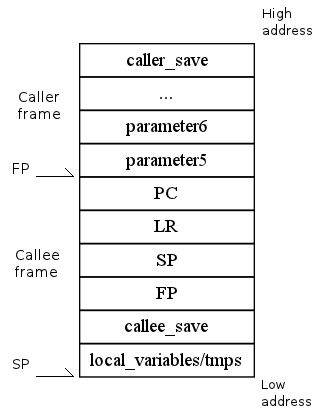
\includegraphics[scale=0.6]{stack_frame.png}
	\label{fig:stackframe}
\end{center}
\end{minipage}
\begin{minipage}{0.4\textwidth}
\begin{center}
	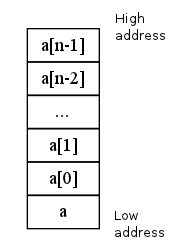
\includegraphics[scale=0.6]{local_array.png}
	\label{fig:localarray}
\end{center}
\end{minipage}
\captionof{figure}{栈帧与局部数组示意图}
\end{center}
FP以上(高地址方向)是调用者的部分栈帧(略去部分和被调用者栈帧相似),其中保存了call save寄存器以及传给被调用者的从第5个到最后一个参数(如果被调用者参数小于等于4,那么省去这一段)。

FP到SP的一段是被调用者的栈帧,其中保存了调用时的PC,返回地址,调用者的栈顶地址和栈帧基址以及callee save寄存器的值。同时,每一个局部变量和没有分配寄存器的临时变量在栈帧中均有位置。


\subsubsection{全局区的维护以及大立即数的处理}
我们将全局变量(或数组)、字符串常量保存在全局区中。由于全局区可能较大,使用基址和偏移量的寻址方式很可能出现偏移量过大不能使用带立即数的访存指令的问题。为此,我们将每个函数需要用到的全局变量的指针保存在该函数的代码段末尾,并分配给它们一个标号。当使用这些标号寻址时,汇编器会自动将寻址方式转换成PC相对寻址。

对于无法使用立即数寻址的三元式中的立即数,我们也将它保存在函数的代码段末尾,通过PC相对寻址将其读入。

例如下述代码:
\begin{lstlisting}
int a,b;
int f()
{
	a=25500;
	b=25500;
}

\end{lstlisting}
我们将生成如下的汇编代码:
\begin{verbatim}
	TODO: assemble code
\end{verbatim}
\section{寄存器分配}
Unicore32采用RISC结构,具有31个通用寄存器,所以对于大部分程序,几乎所有变量都可以保存在这些寄存器中,以减少对内存的读写。因此需要一个方法来给每个变量关联一个寄存器,该方法需要保证能用最节约的方式分配,同时变量之间不能互相污染。

MiniC采用了启发式的图染色寄存器分配算法。该算法依赖于在三元式上进行的活跃变量分析的结果,即需要在某个程序点上每个变量的活跃信息,然后建立一个干涉图$G(V,E)$,其中$V$是变量的集合,$(v_1,v_2)\in E$当且仅当存在某个程序点,使得在此处$v_1$和$v_2$同时活跃。给变量分配寄存器就相当于给这张干涉图着色。

举例如下,对于左图的三元式序列(花括号中是该句处的活跃变量),干涉图为右图:
\begin{center}

\begin{minipage}{0.4\textwidth}
\begin{center}
	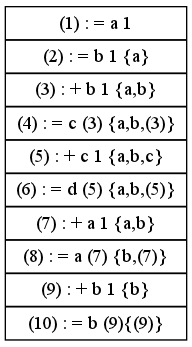
\includegraphics[scale=0.6]{register_allocation_triple.png}
	\label{fig:registerallocationtriple}
\end{center}
\end{minipage}
\begin{minipage}{0.4\textwidth}
\begin{center}
	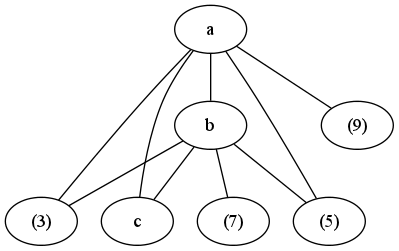
\includegraphics[scale=0.6]{interference_graph.png}
	\label{fig:interferencegraph}
\end{center}
\end{minipage}
\captionof{figure}{寄存器分配示例}
\end{center}
下表给出了不同的可分配寄存器数目的寄存器分配的结果:
\begin{center}
	\begin{tabular}{|l|l|l|}
	\hline
		变量 & 2个可用寄存器 & $\geq$3个可用寄存器 \\
	\hline
		a & 保存在内存 & r6 \\
		b & r5 & r5 \\
		c & r4 & r4 \\
		(3) & r4 & r4 \\
		(5) & r4 & r4 \\
		(7) & r4 & r4 \\
		(9) & r4 & r4 \\
	\hline
	\end{tabular}
	\captionof{table}{寄存器分配示例}
\end{center}
注意到在只有2个可用寄存器时,出现了寄存器不足的情况。对于这种情况MiniC会选择将某些变量保存在内存(即在干涉图中删除该顶点)。这些保存在内存的变量每次引用都需要读取内存;每次赋值都需要写入内存。在\cite{sunjiasu}中介绍的算法采用的选择策略是总选择度数最大的点删除,但是在一些对数组频繁操作的程序实例(如排序算法)中,采用这种策略将会使得数组基址被保存在内存中,使得每次读取数组元素之前要先读取基址,大大影响了性能。为此,MiniC采用了一个改进的策略:\\

%TODO:改进的删点策略
{\it \anchor 有关寄存器分配和活跃变量分析的代码,请参阅:\verb|register_allocation.c|, \verb|live_var_anal.c|}\\
%TODO:三元式转换为目标代码
\section{将三元式转换为目标代码}

\subsection{控制流语句的翻译}

\subsection{翻译过程中对寄存器的保护}

\subsection{立即数的处理}

\section{机器相关优化}
在生成目标代码的过程中,我们已经对一些潜在的代码冗余进行了清理,但是受到中间表示和翻译方法的限制,生成出的目标代码仍有改进的余地,下面介绍我们在目标代码上,配合Unicore32指令系统进行的优化。
\subsection{窥孔优化}
{\it \anchor 有关目标代码上的窥孔优化的代码,请参阅:\verb|peephole.c|}\\
\subsubsection{合并访存语句}
如\verb|a[i] = 1|这样的MiniC语句翻译成的三元式如下:
\begin{center}
	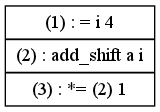
\includegraphics[scale=0.50]{merge_ldst.png}
	\captionof{figure}{合并访存语句示例}
	\label{fig:mergeldst}
\end{center}
根据三元式生成的目标代码为(假设r4中保存着a的基址,r5中保存着i的值):
\begin{verbatim}
add r5, r4, r5<<#2
mov r3, #1
stw r3, [r5+], #0
\end{verbatim}
由于Unicore32提供了“寄存器位移读取(写入)”的指令,这个操作事实上只需要:
\begin{verbatim}
mov r3, #1
stw r3, [r4+],r5<<#2
\end{verbatim}
由于\verb|add|和\verb|stw|可能不连续,逐句生成目标代码时,发现合并的可能较为困难,因此我们扫描生成出的代码,将所有符合上面例子中的情况都进行了合并。

这项简单的优化在循环地对数组访问的情况下对性能的提升比较明显。
\subsubsection{消除冗余的\lstinline|mov|}


\subsection{尾递归优化}
尾递归优化能将符合下面条件的函数调用转化成迭代:
\begin{itemize}
	\item 递归调用
	\item 该调用语句是本函数除返回语句以外的最后一条语句
	\item 该函数没有返回值
\end{itemize}
例如下面的快速排序代码:
\begin{lstlisting}
void qsort(int* data, int begin, int end)
{
	int i,j,tmp;
	if(end <= begin + 1)
		return;
	/* partition routine */
	...
	qsort(data, begin, j - 1);
	qsort(data, j, end);
	return;
}
\end{lstlisting}
注意到第9句的调用符合尾递归条件,因此我们将迭代地处理本次调用:将\verb|data, j, end|分别放在分配给对应参数的寄存器中,然后无条件跳转到函数的开始部分,建立栈帧的语句之后。下面两图对比了生成的目标代码:
\begin{center}
	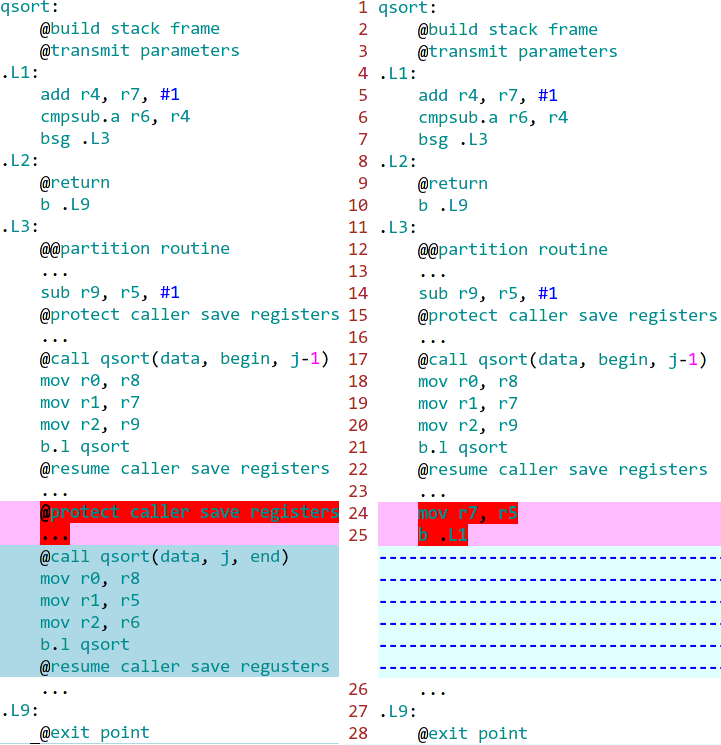
\includegraphics[scale=0.44]{tail_recursion.png}
	\captionof{figure}{尾递归示例}
	\label{fig:tailrecursion}
\end{center}
可以看出,在第二个\verb|qsort|的调用时(24行-30行),进行尾递归优化的程序(右)直接将新值\verb|j|传入被修改的参数\verb|begin|所在的寄存器\verb|r7|中,然后无条件跳转到了函数的正文标号\verb|.L1|。节省了保存、恢复现场以及新调用建立栈帧的指令。\\
{\it \anchor 有关尾递归优化的代码,请参阅:\verb|gen_target_code.c|}\\

\subsection{指令调度}
根据Unicore32指令系统体系结构,除了载入和运算指令可能产生的数据相关无法转发,需要等待一个cycle以外,其它指令的数据相关均已通过转发解决。指令调度的目的是减少甚至消除因载入指令而造成的数据相关。
%TODO:指令调度相关
\paragraph*{算法}

\paragraph*{示例}

